\subsection*{Question 5}

Sample $p(\bm{\theta}|\mathcal{D}_1)$ using \textbf{JAGS} with the same number of iterations (after burnin) as in Q3.

\textbf{a)} Compare your results with the previous ones.

\begin{center}\rule{6cm}{0.4pt}\end{center}

Fitting a JAGS model, we now correctly estimate the growth rate of the number of cancer cells over time as we can notice on the plot below.

\begin{figure}[H]
	\centering
	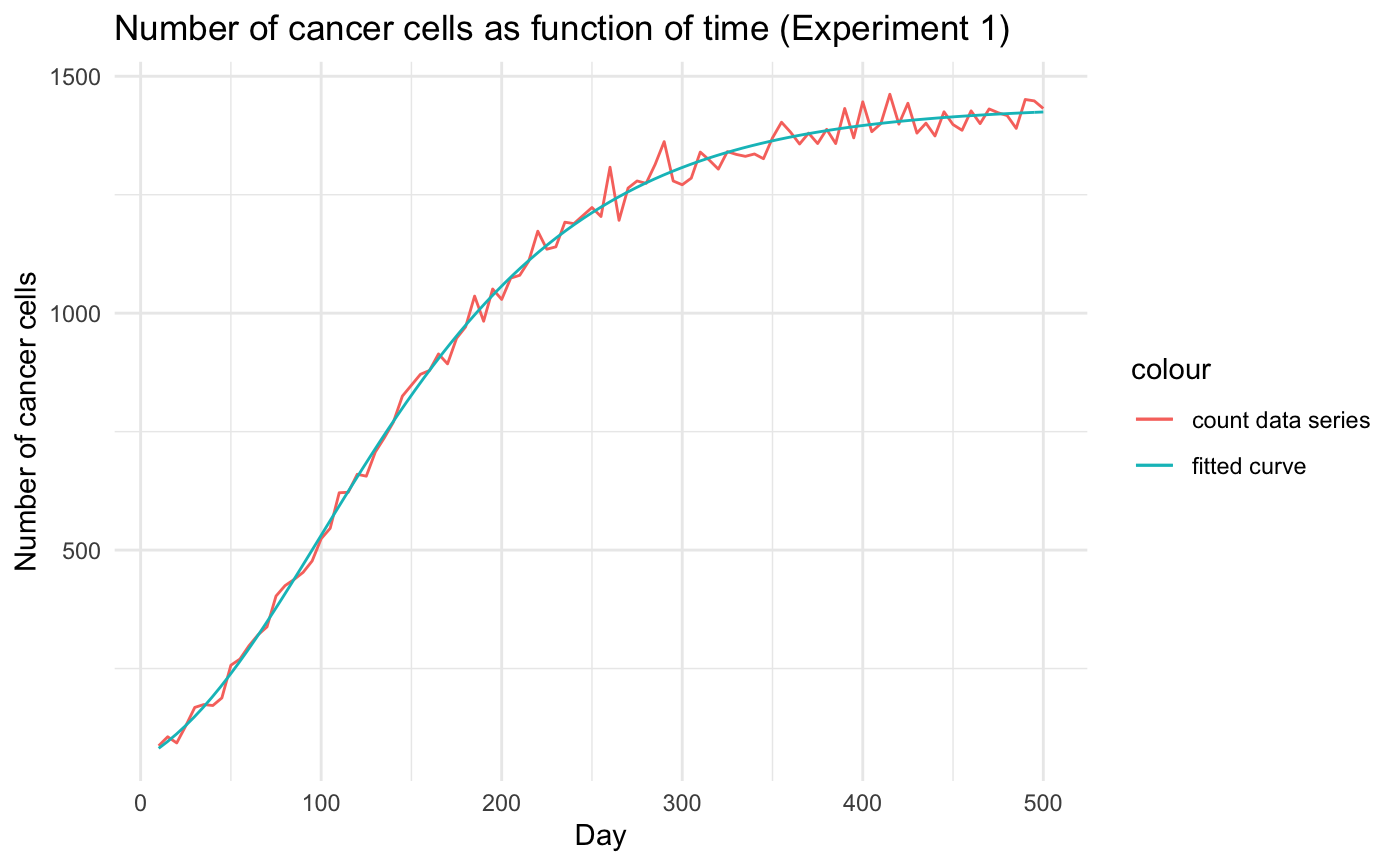
\includegraphics[width=0.7\textwidth]{figures/jags/jags_fitted_curve.png}
	\caption{Comparison of the observed count data series for experiment 1 (\textit{black}) with the fitted curve for $\mu(t)$ (\textit{red})}
	\label{fig:jags-fitted-curve}
\end{figure}

\textbf{b)} Sample the predictive distribution of the number of cancer cells at time $t = +\infty$ and report a point estimates and a credible interval for that quantity.

\begin{center}\rule{6cm}{0.4pt}\end{center}

At time $t = +\infty$, the number of cancer cells follows a Poisson distribution with parameter $\mu = \alpha_0$. Using the predictive posterior obtained above, we can retrieve the $\theta_0$ sample and use it (\textit{knowing that $\theta_0 = \log(\alpha_0)$}) in order to sample from a poisson distribution with parameter $\mu = \alpha_0$. 

We get the following point estimates and $\SI{95}{\percent}$ credible region,
\begin{table}[H]
	\parbox{0.45\linewidth}{
		\centering
		\begin{tabular}{|c|c|c|} \hline 
			Parameter 						& Median 		& Mean \\ \hline 
			$y(t = +\infty)$ 				& $1437$ 		& $1437.596$ \\ \hline
		\end{tabular}
		\caption{Point estimates for the number of cancer cells at $t = +\infty$}
		\label{tab:metropolis-vw-point-estimates-cancer-cells}
	}
	\hfill
	\parbox{0.45\linewidth}{
		\centering
		\begin{tabular}{|c|c|c|} \hline 
			Parameter 						& Lower 		& Upper \\ \hline 
			$y(t = +\infty)$ 				& $1363$  		& $1514$ \\ \hline
		\end{tabular}
		\caption{$\SI{95}{\percent}$ credible region for the number of cancer cells at $t = +\infty$}
		\label{tab:metropolis-vw-credible-region-cancer-cells}
	}
\end{table}

Below, is a density plot of that prediction sample along with the mean shown as vertical dotted blue line.

\begin{figure}[H]
	\centering
	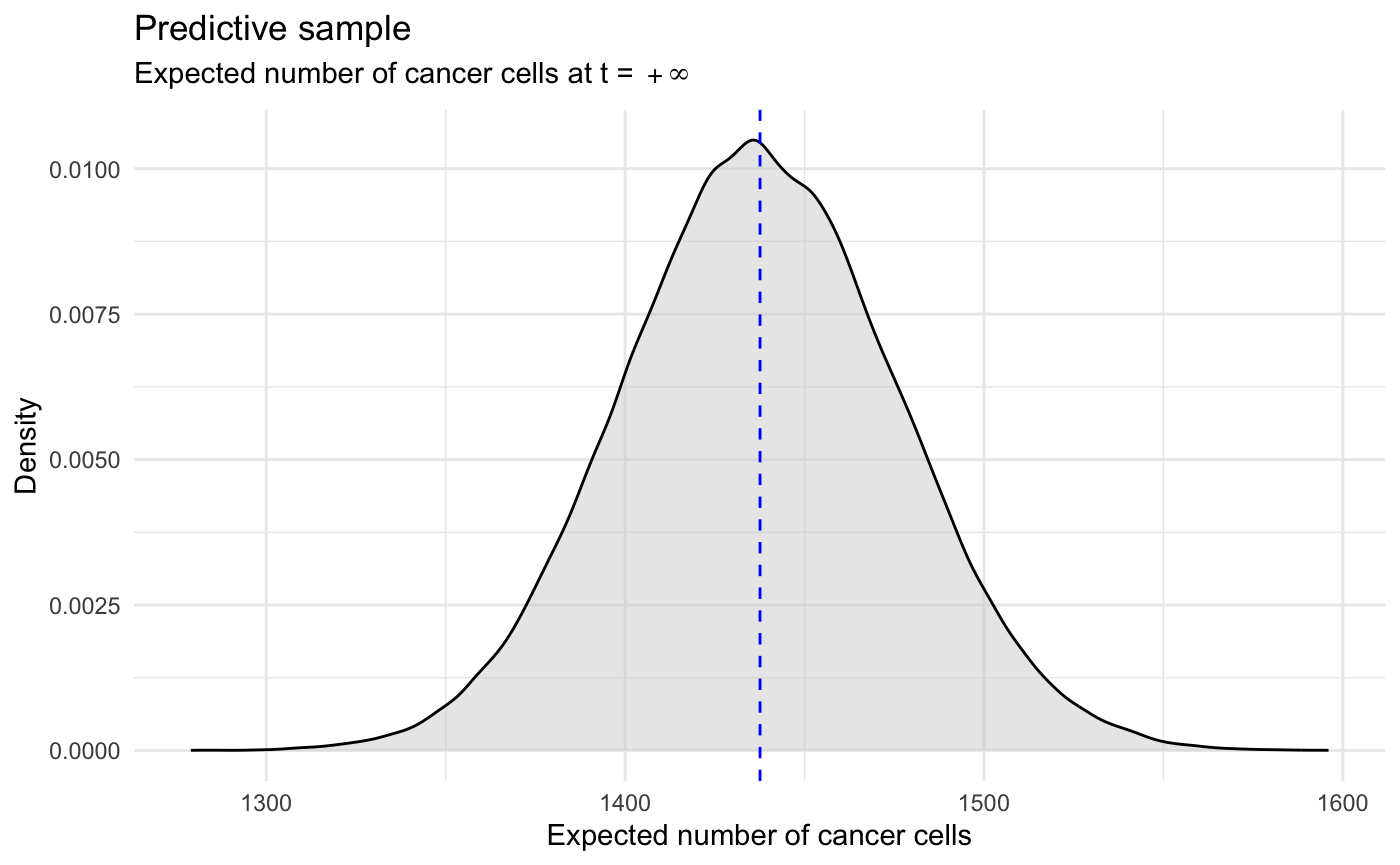
\includegraphics[width=0.7\textwidth]{figures/jags/sample_expected_cancer_cells_tinf.png}
	\caption{Density plot of the sample of the number of cancer cells at t = $\infty$ along with the mean shown as vertical dotted blue line}
	\label{fig:jags-sample-expected-cancer-cells-tinf}
\end{figure}